\documentclass[a4paper, top=10mm]{article}
%for writing from the top
\usepackage{fullpage}
%for math
\usepackage{amsmath}
\usepackage{mathrsfs}
\usepackage{amsthm}
%for images
\usepackage{graphicx}
%for color
\usepackage{xcolor}
%for title
\title{\textbf{\huge{Elves' Shuffling}}}
\author{Enigma n\textsuperscript{o}6}
\date{19\textsuperscript{th} December 2024}

\newtheorem*{hint}{Hint}

\addtolength{\voffset}{-2cm}
\addtolength{\textheight}{5cm}


\begin{document}
	\maketitle
	
	In Santa’s workshop, there are nn elves standing in a line. Each elf is wearing either a red hat or a green hat. They are all aligned together.
	
	The elves are feeling festive and want to rearrange themselves so that all the elves with green hats stand on the left, and all the elves with red hats stand on the right.
	
	To achieve this, they can swap the positions of two adjacent elves in one step.
	
	What is the minimum number of steps required to get all the green-hatted elves grouped on the left and all the red-hatted elves grouped on the right?
	
	The elves are initially standing as follows: RGGRRGRGRGGGRGGG, where:
	\begin{itemize}
		\item "R" represents an elf with a red hat, and
		\item "G" represents an elf with a green hat.
	\end{itemize}
	
	\begin{center}
		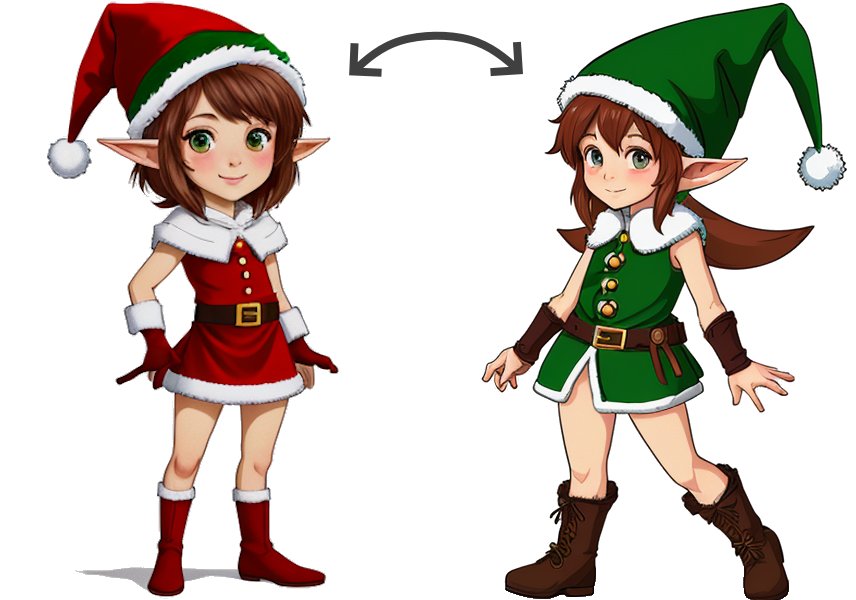
\includegraphics[width=\linewidth]{06elves.png}\\
		Red and green elves swapping positions.
	\end{center}
	
	% Answer: 42
	% https://leetcode.com/problems/separate-black-and-white-balls/?envType=daily-question&envId=2024-10-15
	% with:
	% "RGGRRGRGRGGGRGGG"
	% "1001101010001000"
	
\end{document}